\subsection{Concurrency in the Linux Kernel}
\label{bg:concurrency}

Nowadays, multicore architectures have become mainstream, leading to an ever-increasing demand for concurrency in operating systems. Modern Linux kernel distributions address this demand by providing multiple sources of concurrency~\cite{corbet2005linux}: the kernel can invoke an arbitrary number of entry points from the same module concurrently; a running module process can block and be replaced by another process in the same module; hardware interrupts can be handled concurrently; delayed code execution is the norm; and the user can insert or remove hardware components without rebooting the kernel (known as hot-plugging). All these possibilities can easily lead to serious concurrency issues, such as \emph{data races}, which can be defined as follows:

\begin{definition}
\label{definition:datarace}
A data race occurs when two distinct threads access a shared memory location, at least one of the accesses modifies the location, and there is no mechanism in place to prevent these accesses from being simultaneous.
\end{definition}

Figure~\ref{fig:data_race_example} is an example of a data race between two entry points of a Linux module. The resource \texttt{dev->resource} is shared between the two entry points \texttt{ep1} and \texttt{ep2}. Entry point \texttt{ep1} writes the value 5 to \texttt{dev->resource}, and entry point \texttt{ep2} writes the value 3 to \texttt{dev->resource} if the value of \texttt{dev->resource} is not 5. A data race can occur if \texttt{ep1} and \texttt{ep2} run concurrently: the read and write accesses to the shared resource may execute in arbitrary order leading to nondeterministic behaviour.

\begin{figure}[!h]
\centering
\begin{lstlisting}
static void ep1 (struct shared *dev) {
  dev->resource = 5;
}

static void ep2 (struct shared *dev) {
  if (dev->resource != 5)
    dev->resource = 3;
}
\end{lstlisting}
\caption{Simple data race in a Linux module}
\label{fig:data_race_example}
\end{figure}

\begin{figure}[!h]
\centering
\noindent\begin{minipage}{.95\textwidth}
\begin{lstlisting}
static void ep1 (struct shared *dev) {
  lock(&dev->lock);
  dev->resource = 5;
  unlock(&dev->lock);
}

static void ep2 (struct shared *dev) {
  lock(&dev->lock);
  if (dev->resource != 5)
    dev->resource = 3;
  unlock(&dev->lock);
}
\end{lstlisting}
\end{minipage}
\caption{Using locks to eliminate the data race}
\label{fig:lock_example}
\end{figure}

The most common technique for eliminating data races is using a \emph{locking} mechanism. Locking a set of program statements that access a shared resource creates a \emph{critical section}, i.e. source code that cannot be executed by more than one thread simultaneously. Figure~\ref{fig:lock_example} shows how to use a lock to eliminate the data race in the previous example.

Lock-based synchronisation is a powerful tool for preventing data races in drivers, but careless use of locks has multiple pitfalls~\cite{sutter2005software}. Coarse-grained locking can severely hurt performance, because it limits the opportunity for concurrency. On the other hand, fine-grained locking can easily lead to \emph{deadlocks}, a system-halting situation in which no active thread can progress, because it is waiting to acquire a lock that is held by another blocked thread. Although the Linux kernel provides sophisticated lock-free synchronisation mechanisms~\cite{corbet2005linux}, in this work we focus on locks.

\subsection{Reasoning about Thread Interleavings}
\label{bg:happensbefore}

A fundamental concept in concurrency analysis is Lamport's \emph{happens-before} relation~\cite{lamport1978time}, which denotes a partial-order between all events during the execution of a concurrent program. Happens-before can be defined as follows:

\begin{definition}
\label{definition:datarace}
Let $E_1$ and $E_2$ be two events during a program's concurrent execution. If $E_1$ and $E_2$ are in the same thread and $E_1$ occurs before $E_2$, or if $E_1$ and $E_2$ are in different threads and there is a synchronisation mechanism (e.g. locking) that prevents a thread schedule in which $E_2$ occurs before $E_1$, then $E_1 \rightarrow E_2$, where the symbol $\rightarrow$ denotes the happens-before relation.
\end{definition}

Happens-before is transitive, i.e. for any three events $E_1$, $E_2$ and $E_3$, if $E_1 \rightarrow E_2$ and $E_2 \rightarrow E_3$, then $E_1 \rightarrow E_3$. If two events $E_1$ and $E_2$ occur in different threads, and neither $E_1 \rightarrow E_2$, nor $E_2 \rightarrow E_1$ holds, then $E_1$ and $E_2$ happen concurrently, which indicates a data race if the two events access the same shared resource and at least one of the accesses is a modifier.

\begin{figure}[htbp]
\centering
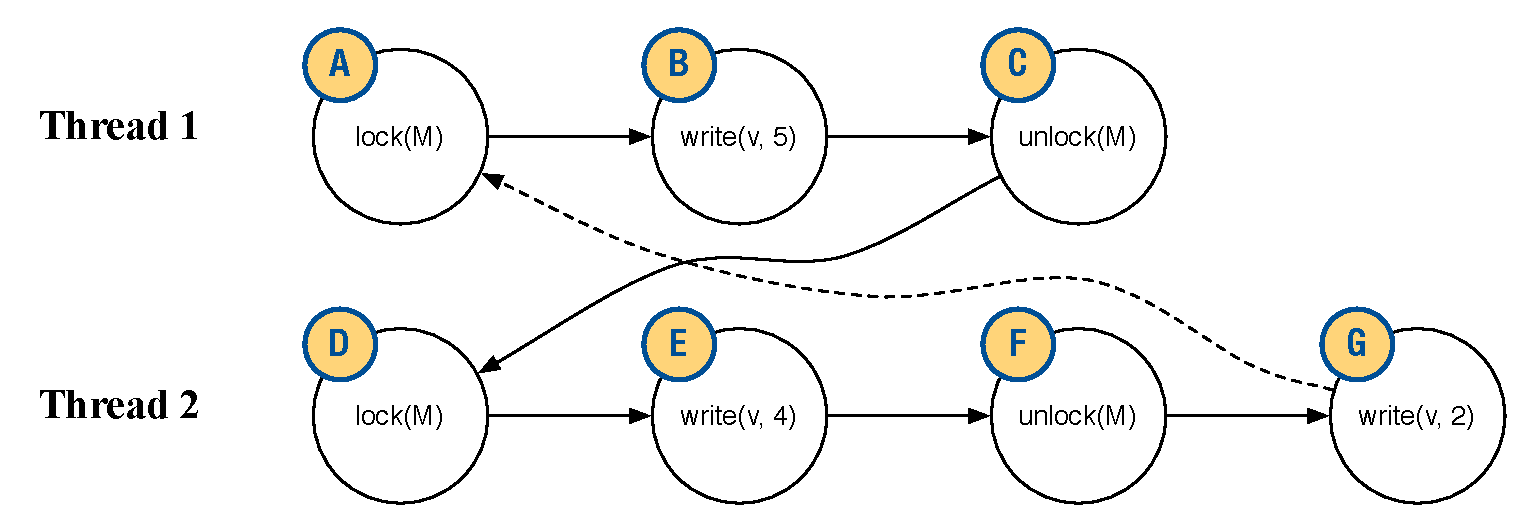
\includegraphics[width=1\linewidth]{img/happens_before.pdf}
\caption{Example showcasing the main limitation of happens-before}
\label{fig:happens_before}
\end{figure}

Figure~\ref{fig:happens_before} shows an example of applying happens-before reasoning in two concurrently running entry points. Each of the three statements $\{A, B, C\}$ in thread 1 is executed before the next one, and thus all of them are ordered by the happens-before relation. The same applies for each of the four statements $\{D, E, F, G\}$ in thread 2. Statement $C$ in thread 1 releases the lock, and subsequently allows $D$ in thread 2 to acquire the same lock. Thus, $C \rightarrow D$. This means that for this specific thread interleaving the set of statements $\{A, B, C\}$ happens before the set of statements $\{D, E, F, G\}$.

The above example also showcases the main limitation of happens-before. If the technique explores \emph{only} this specific thread interleaving, it will miss a potential data race between statements $B$ and $G$, because $B \rightarrow G$ in this specific schedule. Thus, a tool based on happens-before requires a scheduler that produces as many different thread interleavings as possible to increase execution path coverage~\cite{savage1997eraser}. Achieving full coverage with tools based on happens-before is infeasible though, because of the exponential number of possible thread interleavings in realistic concurrent programs. Furthermore, attempting to explore a large number of thread schedules quickly leads to scalability issues~\cite{musuvathi2008finding}, a problem known as state space explosion. Thus, previous work based on happens-before typically explore paths under a certain bound, such as the number of allowed context switches~\cite{qadeer2004kiss}.

\subsection{Reasoning about Locksets}
\label{bg:lockset}

An alternative approach to happens-before, known as \emph{lockset analysis}, resolves around reasoning about the locking behaviour of concurrent programs. Lockset analysis has its roots in Eraser~\cite{savage1997eraser}, a dynamic data race detector that tracks the set of locks that \emph{consistently} protect a memory location during program execution. If that lockset ever becomes empty, the analysis reports a potential data race on that memory location. This is because an inconsistent lockset suggests that a memory location \emph{may} be accessed simultaneously by two or more threads.

\begin{figure}[htbp]
\centering
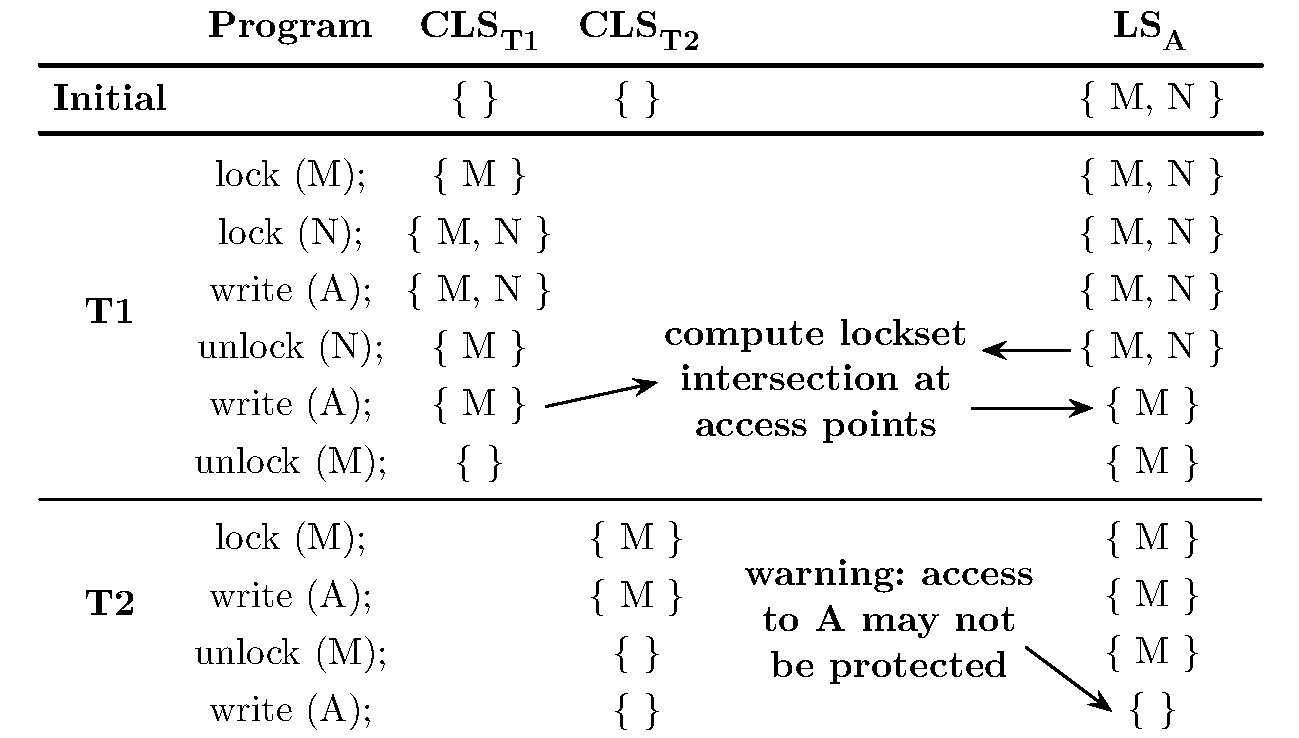
\includegraphics[width=1\linewidth]{img/lockset.pdf}
\caption{Applying lockset analysis on a thread of a concurrent program}
\label{fig:locksets}
\end{figure}

Figure~\ref{fig:locksets} shows an example of applying lockset analysis on a thread of a concurrent program. Lockset analysis starts by creating one lockset for each thread $T$ in the program, called current lockset of $T$ or $CLS_T$, and one lockset for each shared variable $v$, called lockset of $v$ or $LS_v$. In this example we analyse only one thread and only one shared variable and thus there are two such locksets: Current Lockset ($CLS$) and Lockset A ($LS_A$). Initially, $CLS$ is empty, because it represents the set of locks before the program starts executing, which is the empty set $\{ \}$. Likewise, $LS_A$ starts as the set of all existing locks in the program, which in this case is $\{M, N\}$. Lockset analysis then proceeds as follows:

\begin{enumerate}
\item In each \emph{lock} and \emph{unlock} operation, update ($CLS$) with the currently held locks.
\item In each shared variable access, update ($LS_A$) with the intersection of the latest ($CLS$) and the ($LS_A$) of the previous statement.
\item If ($LS_A$) ever becomes empty, then report that access to $A$ is unprotected.
\end{enumerate}

Lockset analysis avoids reasoning about arbitrary thread interleavings, and thus has the potential to scale well in realistic concurrent programs. The technique, though, suffers from imprecision (i.e. can report many false bugs), because a violation of the locking discipline does not always correspond to a real data race~\cite{savage1997eraser, pozniansky2003efficient, o2003hybrid, elmas2007goldilocks, flanagan2009fasttrack}. Furthermore, as a classic dynamic analyser, Eraser's bug finding ability is limited to the execution paths that the tool explores. To counter these limitations, we apply the idea of Eraser's lockset analysis in a static verification context.